\chapter{\topos{}的内语言: 从语法到语义}

\philoquote{
    A mathematical statement is just a story you tell about some devices. Some of those stories are clever, some are stupid; some of those stories are true, some others are false. Doing mathematics is telling clever stories which are true.\footnotemark
}{
    Francis Borceux, \cite{HCA3}
}
\footnotetext{一句数学陈述不过是你对某些东西讲的一个故事. 这些故事有的妙, 有的蠢, 有的真, 有的假. 做数学就是要讲出又妙又真的故事.}

我们曾提到\topos{}中有一种\emph{内语言} (internal language) 可用来进行推理, 本章介绍这种语言, 以及它在各个数学分支中的应用.
建议不熟悉数理逻辑的读者在本章之前先阅读附录 \ref{logic-appendix}.

\section{Mitchell--B\'enabou 语言}

\label{Mitchell--Benabou-language}

本节描述一种重要的语言, 称作 \emph{Mitchell--B\'enabou 语言}; 它是由给定的\topos{} $\mathsf C$ 定义出的一种一阶语言, 其特点是利用子对象分类器 $\Omega$, 将\emph{公式}一视同仁地解释为 $\Omega$ 类型的\emph{项}. 使用这种语言, 可将\topos{}中的对象在语法上当作集合一样处理.

\begin{definition}
    {(类型)}
    Mitchell--B\'enabou 语言中的\emph{类型}是 $\mathsf C$ 的对象.
\end{definition}


%\begin{itemize}
%	\item 类型 $X$ 的\emph{项}被解释为指向 $X$ 的态射, 而\emph{公式}被解释为 $\Omega$ 类型的项;
%	项 (公式) 的定义域代表此项 (公式) 中自由变量的类型.
%	例如, 当类型 $X$ 的一个项含有自由变量 $y\colon Y, z\colon Z$ 时, 该项解释为一个态射 $Y\times Z \to X$.
%	\item 
%	\item 
%\end{itemize}


\begin{definition}
	{(函数符号, 关系符号)}
	Mitchell--B\'enabou 语言中的\emph{函数符号} $f\colon A_1\cdots A_n \to B$ 是 $\mathsf C$ 中的态射
	$$f\colon A_1\times\cdots\times A_n\to B.$$
	特别地, 类型 $X$ 的\emph{常量} (零元函数) 是态射 $1 \to X$, 也即对象 $X$ 的\emph{整体元素}.
	
	Mitchell--B\'enabou 语言中的\emph{关系符号} $R\hookrightarrow A_1\cdots A_n$ 是 $\mathsf C$ 中的态射
	$$
	R\colon A_1\times\cdots\times A_n \to \Omega,
	$$
	也即 $A_1\times\cdots\times A_n$ 的子对象, 其直观为 ``满足关系 $R$ 的元素构成的子集''.
	特别地, 原子命题 (零元关系) 是态射 $1\to\Omega$, 也即\emph{真值}.
	
	%我们看到, 函数符号与项被解释成了同一种东西. 这是有道理的, 因为\emph{项}在这里就是其自由变量的函数.
\end{definition}

至此, Mitchell--B\'enabou 语言已经定义完成. 接下来我们归纳地给出这种语言中的项和公式的\emph{解释} (interpretation).

%\begin{definition}
%    {(变量的解释)}
%    
%\end{definition}


%\begin{definition}
%	{(等式)}
%	
%\end{definition}


\begin{definition}
	{(项的解释)}
	\begin{itemize}
		\item (变量)
		类型 $X$ 的一个\emph{变量} (可视为含一个自由变量的项) 解释为恒等态射 $\operatorname{id}\colon X \to X$.
		\item (函数取值)
		对于函数符号 $f\colon X \to Y$ 与类型 $X$ 的项 $\sigma\colon U \to X$, $f(\sigma)$ 解释为复合 $f\circ\sigma \colon U \to Y$.
	\end{itemize}
\end{definition}

\begin{remark}
	{(一般元素)}
	设 $x$ 是类型 $X$ 的一个变量.
	假若我们证明了含变量 $x$ 的公式 $\phi(x)$,
	那么对 $X$ 的任意具体的项 $x_0$, 就有 $\phi(x_0)$ 成立.
	在 Mitchell--B\'enabou 语言中, $x\in X$ 被解释为 $\operatorname{id}\colon X\to X$, 它可视为对象 $X$ 的\emph{一般元素} (generic element) (这里元素的含义是广义元素, 即态射 $?\to X$), 因为对任意态射 $f\colon X\to Y$, 只要给定了 $f$ 在广义元素 $\operatorname{id}\colon X\to X$ 上的值 $f\circ\operatorname{id}$, 就确定了 $f$ 在任何广义元素 $x_0\colon U\to X$ 上的值 $f\circ x_0$. 这是平凡的.
\end{remark}

特别地, 使用取值映射 $\operatorname{ev}\colon Y^X\times X\to Y$ (定义 \ref{evaluation-map}),
可将 $Y^X$ 类型的项 (内语言中的 ``函数'') $\theta\colon V\to Y^X$
作用于 $X$ 类型的项 $\sigma \colon U \to X$,
得到 $Y$ 类型的项
% https://q.uiver.app/#q=WzAsMyxbMCwwLCJWXFx0aW1lcyBVIl0sWzEsMCwiWV5YXFx0aW1lcyBYIl0sWzIsMCwiWSJdLFswLDEsIihcXHRoZXRhLFxcc2lnbWEpIl0sWzEsMiwiXFxvcGVyYXRvcm5hbWV7ZXZ9Il1d
\[\theta(\sigma)\colon
\begin{tikzcd}[ampersand replacement=\&]
	{V\times U} \& {Y^X\times X} \& Y.
	\arrow["{(\theta,\sigma)}", from=1-1, to=1-2]
	\arrow["{\operatorname{ev}}", from=1-2, to=1-3]
\end{tikzcd}\]

例如, 考虑成员关系 (例 \ref{membership-relation}) ${\in_X} \colon \Omega^X\times X \to \Omega$,
可对 $PX=\Omega^X$ 类型的项 (内语言中的 ``子集'') $\eta\colon V \to \Omega^X$ 与 $X$ 类型的项 $\sigma\colon U\to X$ 定义 $\Omega$ 类型的项
% https://q.uiver.app/#q=WzAsMyxbMCwwLCJWXFx0aW1lcyBVIl0sWzEsMCwiXFxPbWVnYV5YXFx0aW1lcyBYIl0sWzIsMCwiXFxPbWVnYSJdLFswLDEsIihcXGV0YSxcXHNpZ21hKSJdLFsxLDIsIlxcaW5fWCJdXQ==
\[
(\sigma \in \eta) \colon 
\begin{tikzcd}[ampersand replacement=\&]
	{V\times U} \& {\Omega^X\times X} \& \Omega.
	\arrow["{(\eta,\sigma)}", from=1-1, to=1-2]
	\arrow["{\in_X}", from=1-2, to=1-3]
\end{tikzcd}\]

\begin{definition}
	{(公式)}
	\begin{itemize}
		\item
		(等式) 对于类型 $X$ 的两个项 $\sigma\colon U \to X$, $\tau\colon V \to X$, \emph{等式} $\sigma = \tau$ 被解释为 $\Omega$ 的项
		% https://q.uiver.app/#q=WzAsMyxbMCwwLCJVXFx0aW1lcyBWIl0sWzEsMCwiWFxcdGltZXMgWCJdLFsyLDAsIlxcT21lZ2EiXSxbMCwxLCIoXFxzaWdtYSxcXHRhdSkiXSxbMSwyLCJcXGNoaV97XFxEZWx0YX0iXV0=
		\[\begin{tikzcd}[ampersand replacement=\&]
			{U\times V} \& {X\times X} \& \Omega.
			\arrow["{(\sigma,\tau)}", from=1-1, to=1-2]
			\arrow["{\chi_{\Delta}}", from=1-2, to=1-3]
		\end{tikzcd}\]
		回忆 $\chi_{\Delta}$ 是对角线 $\Delta\colon X\to X\times X$ 的特征函数 (例 \ref{diagonal}), 它表达的正是 $X$ 上的相等关系.
	\end{itemize}
\end{definition}

\begin{definition}
	{(公式确定的子对象)}
	对公式 $\phi(x)$, 设其解释为 $p\colon X\to\Omega$, 定义 $X$ 的子对象 $\{x\in X \mid \phi(x)\}$ (或简记为 $\{x\mid \phi(x)\}$) 为如下的拉回.
	\[
	\begin{tikzcd}
		\{x\mid \phi(x)\}\ar[r]\ar[d] & 1\ar[d] \\
		X \ar[r,"p"'] & \Omega
	\end{tikzcd}
	\]
\end{definition}



\subsection{内语言中的逻辑}

\todo{挪到第一章}

在一个\topos{}中, $\Omega$ 是代表真值的类型, 从而逻辑运算可表示为与 $\Omega$ 相关的态射. 前面提到的 ``真'' $\top \colon 1 \to \Omega$ 属于此列.

\subsection{假, 非}

\begin{definition}
	{(假)}
	\emph{假} (false) $\bot \colon 1 \to \Omega$ 是 子对象 $0\to 1$ 的特征函数, 即下图是子对象的拉回.
	% https://q.uiver.app/#q=WzAsNCxbMCwwLCIwIl0sWzAsMSwiMSJdLFsxLDEsIlxcT21lZ2EiXSxbMSwwLCIxIl0sWzAsMV0sWzAsM10sWzEsMiwiXFxib3QiLDJdLFszLDIsIlxcdG9wIl1d
	\[\begin{tikzcd}[ampersand replacement=\&]
		0 \& 1 \\
		1 \& \Omega
		\arrow[from=1-1, to=2-1]
		\arrow[from=1-1, to=1-2]
		\arrow["\bot"', from=2-1, to=2-2]
		\arrow["\top", from=1-2, to=2-2]
	\end{tikzcd}\]
\end{definition}

\begin{definition}
	{(非)}
	\emph{非} (not) $\neg\colon \Omega\to\Omega$ 是\emph{假} $\bot\colon 1 \to\Omega$ 的特征函数, 即下图是子对象的拉回.
	% https://q.uiver.app/#q=WzAsNCxbMCwwLCIxIl0sWzAsMSwiXFxPbWVnYSJdLFsxLDEsIlxcT21lZ2EiXSxbMSwwLCIxIl0sWzAsMSwiXFxib3QiLDJdLFswLDNdLFsxLDIsIlxcbmVnIiwyXSxbMywyLCJcXHRvcCJdXQ==
	\[\begin{tikzcd}[ampersand replacement=\&]
		1 \& 1 \\
		\Omega \& \Omega
		\arrow["\bot"', from=1-1, to=2-1]
		\arrow[from=1-1, to=1-2]
		\arrow["\neg"', from=2-1, to=2-2]
		\arrow["\top", from=1-2, to=2-2]
	\end{tikzcd}\]
\end{definition}

\subsection{且}

\begin{definition}
	{(且)}
	
\end{definition}

\begin{definition}
	{(真值, 内语言定义)}
	公式 $\varphi$ 的\emph{真值}是集合
	$$
	\{x:1 \mid \varphi\} \in \Omega,
	$$
	其中 $x$ 是不出现在 $\varphi$ 中的变量.
\end{definition}

\section{模态与层化}

本节讨论模态 (\ref{appendix-modal-logic}), Lawvere--Tierney 拓扑与层化.

首先我们重新定义 Lawvere--Tierney 拓扑 (定义 \ref{Lawvere--Tierney-topology}).

\begin{definition}
	{(Lawvere--Tierney 拓扑, 内语言定义)}
	满足如下条件的映射 $\square\colon \Omega\to\Omega$ 称作\emph{Lawvere--Tierney 拓扑}, 或\emph{模态}:
	\begin{itemize}
		\item $\varphi\Rightarrow \square \varphi$;
		\item $\square\square\varphi \Rightarrow \square\varphi$;
		\item $\square(\varphi \land \psi) \Leftrightarrow \square\varphi\land \square\psi$.
	\end{itemize}
\end{definition}

\begin{example}
	{}
	如下映射都是 Lawvere--Tierney 拓扑:
	\begin{itemize}
		\item $\square\varphi = (\mu\Rightarrow\varphi)$;
		\item $\square\varphi = (\nu\lor\varphi)$;
		\item $\square\varphi = \neg\neg\varphi$.
	\end{itemize}
\end{example}

\begin{definition}
	{(分离性与层条件, 内语言定义)}
	对于给定的Lawvere--Tierney 拓扑 $\square$, 称集合 $F$ $\square$-\emph{分离}是指
	$$
	\forall x,y:F. \square (x=y) \Rightarrow x=y.
	$$
	称集合 $F$ 为\emph{层}是指 $F$ 分离, 且
	$$
	\forall S \subset F. \square (\text{$S$ 是单元集}) \Rightarrow \exists x:F.\square(x\in S).
	$$
\end{definition}

一个集合 $\square$-分离

\todo{层化}


%\section{几何理论}

\section{层语义}

\todo{stack semantics}

% https://ncatlab.org/nlab/show/stack+semantics

%\todo{将综合可计算性理论, 综合微分几何, 综合代数几何变成本章的节}

\section{非标准分析, 滤商与超滤范畴}

\emph{非标准分析}起源于对无穷小与极限等概念的重新审视. 不同于 Cauchy--Weierstrass 的 $\varepsilon$-$\delta$ 方法, 它将无穷小量视为扩充实数集中实实在在的对象. 一种称作\emph{传达原理}的工具提供了经典分析与非标准分析之间的桥梁.

\subsection{基本概念}

\begin{definition}
	{(超滤)}
	Boole 代数 $B$ 上的\emph{超滤}是 Boole 代数同态 $B\to \{\bot,\top\}$ 下 $\top$ 的原像. 超滤 $\mathcal F$ 也可由如下等价的条件之一定义:
	\begin{itemize}
		\item $\mathcal F$ 是极大的真滤子;
		\item $\mathcal F$ 是真滤子, 且对任意 $a\in B$, 要么 $a\in\mathcal F$, 要么 $\neg a\in \mathcal F$.
	\end{itemize}
	集合 $S$ 上的超滤是指 Boole 代数 $2^S$ 上的超滤.
\end{definition}

\begin{remark}
	{}
	一个集合上超滤构成的空间是其子集 Boole 代数的 Stone 空间, 这是代数--几何对偶的一例. 参见定义 \ref{points-of-locale} 及其后的注.
\end{remark}

\subsection{滤商}

\subsection{超滤范畴}

\section{可计算性理论与有效意象}

有效意象 (effective topos) $\mathsf {Eff}$ 是用于研究可计算性理论的范畴, 或用一种诗意的表达, 是 ``可计算数学的世界'' (相对于 $\mathsf {Set}$ 是 ``通常数学的世界'').



\section{综合微分几何与光滑无穷小分析}

\subsection{综合微分几何的理论}

我们首先在本小节叙述一种偏向语法的 (或公理化的) 理论, 而暂时不关心这个理论是否存在一个模型. 我们将看到这种理论比通常的微分几何更加符合直观.

\begin{axiom}
	{(空间)}
	综合微分几何所谓的\emph{空间} (或称\emph{集合}) 是一个固定的\topos{} $\mathsf E$ 中的对象; \emph{光滑映射} (或称\emph{映射}) 是 $\mathsf E$ 中的态射.
\end{axiom}

\begin{axiom}
	{(直线)}
	综合微分几何所谓的\emph{直线}是 $\mathsf E$ 中一个固定的环 $R$.
\end{axiom}

\begin{remark}
	{}
	字母 $R$ 提示了这个对象与通常微分几何的对象 $\mathbb{R}$ 在直观上的相似性, 但它与 $\mathbb{R}$ 有不同的性质, 如 ``幂零无穷小量'' 的存在性. 因此, 我们不能要求 $R$ 是域.
\end{remark}

\begin{definition}
	{(直线上原点的一阶无穷小邻域)}
	定义 $R$ 上 ``原点的一阶无穷小邻域''
	$$
	D = \{x \in R \mid x^2 = 0\}.
	$$
\end{definition}

\begin{example}
	{(相切曲线的共同切向量)}
	平面 $R^2$ 上的直线 $y=0$ 与圆 $x^2 + (y-1)^2 = 1$ 的交集是 $D$. 这是因为将 $y=0$ 代入圆的方程, 就得到 $x^2 + 1 = 1$, 也即 $x^2 = 0$.
	
	\begin{center}
		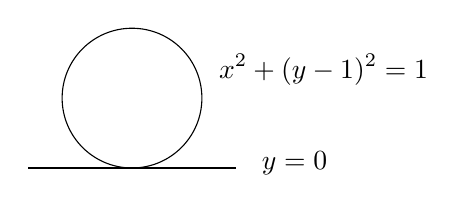
\begin{tikzpicture}[x=0.75pt,y=0.75pt,yscale=-1,xscale=1]
			%uncomment if require: \path (0,300); %set diagram left start at 0, and has height of 300
			
			%Straight Lines [id:da9022525264933119] 
			\draw    (44,106) -- (144,106) ;
			%Shape: Circle [id:dp5620106547865036] 
			\draw   (60.33,72.33) .. controls (60.33,53.74) and (75.41,38.67) .. (94,38.67) .. controls (112.59,38.67) and (127.67,53.74) .. (127.67,72.33) .. controls (127.67,90.93) and (112.59,106) .. (94,106) .. controls (75.41,106) and (60.33,90.93) .. (60.33,72.33) -- cycle ;
			
			% Text Node
			\draw (155.33,97) node [anchor=north west][inner sep=0.75pt]   [align=left] {$\displaystyle y=0$};
			% Text Node
			\draw (134.67,50) node [anchor=north west][inner sep=0.75pt]   [align=left] {$\displaystyle x^{2} +( y-1)^{2} =1$};
		\end{tikzpicture}
	\end{center}
	
	直观上, 直线与圆相切, 两者在相切处有一条公共的 ``无穷小线段''. 更一般地, 任意两条相切的曲线都有一条公共的形如 $D$ 的无穷小线段, 这便是两条曲线共同的切向量.
\end{example}

\paragraph{Kock--Lawvere 公理与导数}

~

\begin{axiom}
	{(Kock--Lawvere 公理)}
	对任意映射 $f \colon D \to R$, 存在唯一的 $a,b\in R$,
	使得
	$$
	f(d) = a + d\cdot b,\quad\forall d\in D.
	$$
	换言之, 作为 $R$-代数有
	$$
	\operatorname{Hom}(D,R) \simeq R[x]/(x^2).
	$$
\end{axiom}

Kock--Lawvere 公理反映了如下的直观: $R$ 上的一个函数在一个很小的邻域上近乎是一次函数.
由此, 我们立刻得到如下的推论.

\begin{propdef}
	{(导函数)}
	对任意函数 $f\colon R\to R$, 存在唯一的函数 $f' \colon R \to R$ 满足
	$$
	f(x+d) = f(x) + d \cdot f'(x),\quad \forall x\in R\,\forall d\in D.
	$$
	称 $f'$ 为 $f$ 的\emph{导函数}. 归纳地定义 $k$ 阶导数 $f^{(k)}(x)$.
\end{propdef}

任何函数都是任意次可导的.

\paragraph{Weil 代数与无穷小几何对象}

~

无穷小线段 $D$ 对应代数 $R[x]/(x^2)$. 一般地, 在代数--几何对偶中与无穷小几何对象相对应的代数是 \emph{Weil 代数}.
\begin{definition}
	{(Weil 代数)}
	Weil 代数是形如 $W = R \oplus J$ 的 $R$-代数,
	其中 $J$ 是有限生成自由 $R$-模,
	且为幂零理想.
\end{definition}

\begin{definition}
	{(Weil 代数的谱)}
	对于 Weil 代数 $W$, 定义 $W$ 的\emph{谱}为 $R$-代数同态的空间
	$$
	\operatorname{Spec}W = \operatorname{Hom}_{R\mathsf {Alg}}(W,R),
	$$
	称之为\emph{无穷小几何对象}.
\end{definition}

\begin{example}
	{(常见的无穷小几何对象)}
	\begin{itemize}
		\item 点 $$\text{pt} \simeq \{x\in R\mid x=0\} = \operatorname{Spec} R;$$
		\item 无穷小线段的平方 $$D^2 \simeq \{(x,y)\in R^2 \mid x^2=y^2=0\} = \operatorname{Spec}R[x,y]/(x^2,y^2);$$
		\item $R^2$ 上原点的一阶无穷小邻域 $$D(2) := \{(x,y)\in R^2\mid x^2=xy=y^2=0\} = \operatorname{Spec}R[x,y]/(x^2,xy,y^2);$$
		\item 高阶无穷小邻域
		$$
		D_k := \{x\in R\mid x^{k+1}=0\} = \operatorname{Spec}R[x]/(x^{k+1})\, (k=1,2,3,\cdots).
		$$
	\end{itemize}
\end{example}

前面介绍的 Kock--Lawvere 公理可表述为 $\operatorname{Hom}(\operatorname{Spec}R[x]/(x^2),R) \simeq R[x]/(x^2)$. 类似地有如下公理.

\begin{axiom}
	{(Kock--Lawvere 公理)}
	对于 Weil 代数 $W$, 有
	$$
	\operatorname{Hom}(\operatorname{Spec}W,R)\simeq W.
	$$
\end{axiom}

\begin{remark}
	{(Weil 代数与 Kock--Lawvere 公理的直观)}
	设 $W=R\oplus J$ 是 Weil 代数. 投影 $W \to R$ 对应点 $\text{pt}$ 到无穷小几何对象 $\operatorname{Spec}W$ 的\emph{原点}的嵌入 $$\text{pt} = \operatorname{Spec} R \to \operatorname{Spec}W.$$
	Kock--Lawvere 公理说的是 Weil 代数 $W$ 等同于 $\operatorname{Spec}W$ 上的函数代数. 投影 $W\to R$ 可视为 $\operatorname{Spec}W$ 上的函数在原点处取值; 理想 $J$ 是投影 $W\to R$ 的核, 可视为在原点取值为 $0$ 的函数的集合.
	要求 $J$ 为\emph{幂零}理想, 也即要求在原点取值为 $0$ 的函数都幂零, 直观上说明 $\operatorname{Spec}W$ 是 ``无穷小'' 的.
\end{remark}

\subsection{综合微分几何的模型}



\begin{definition}
	{}
	
\end{definition}

\section{量子理论与 Bohr 意象}



\subsection{$C^*$-代数, 经典语境与 Bohr 景}

一般而言, 量子系统是由 $C^*$-代数表示的.

\begin{remark}
    {(约定)}
    约定本章中的 ``代数'' 指含幺结合代数, 且代数的同态保持幺元.
\end{remark}

\begin{definition}
    {($C^*$-代数)}
    \emph{$C^*$-代数}是 $\mathbb{C}$ 上的 Banach 代数 $\big(\mathcal A,\|{-}\|\big)$,
    带有 ``伴随'' 运算 $(-)^*\colon \mathcal A \to \mathcal A$,
    满足对任意 $x\in \mathcal A$,
    \begin{itemize}
        \item $(x^*)^*=x$,
        \item $(xy)^*=y^*x^*$,
        \item $(\lambda x)^*=\bar\lambda x^*\,(\lambda\in\mathbb{C})$,
        \item $\|x^* x\|=\|x\|\|x^*\|=\|x\|^2$.
    \end{itemize}
    $C^*$-代数的 $*$-子代数是指关于 $(-)^*$ 封闭的子代数.
\end{definition}

\begin{example}
    {}
    对于 Hilbert 空间 $H$, $H$ 上的有界线性算子的代数 $\mathcal B(H)$ 是 $C^*$-代数, 其中 $x^*$ 是 $x$ 的伴随算子. 事实上, 每个 $C^*$-代数都同构于某个形如 $\mathcal B(H)$ 的代数的 $*$-子代数, 因此后者也可作为 $C^*$-代数的一种具体定义.
\end{example}

下面我们固定一个 $C^*$-代数 $\mathcal A$.

\begin{definition}
    {(可观测量)}
    $C^*$-代数中的自伴元素是指满足 $x^*=x$ 的元素; 自伴元素又称\emph{可观测量} (observable).
\end{definition}

Heisenberg 不确定性原理表明, 不交换的可观测量不可同时确定, 而一族相交换的可观测量可以同时确定. 因此我们格外关注那些交换的子代数.

\begin{definition}
    {(经典语境)}
    称 $\mathcal A$ 的一个交换 $*$-子代数为一个\emph{经典语境} (classical context).
    记 $\mathsf C(\mathcal A)$ 为 $\mathcal A$ 的交换 $*$-子代数在包含关系下构成的偏序集.
\end{definition}

\begin{remark}
    {}
    语境这个名字的含义是, 一个可观测量只在某些特定的语境 (也就是包含它的那些语境) 下才有确定的值. 在一个固定的语境中, 可观测量的表现无异于一个经典系统.
\end{remark}

这里我们稍微偏题, 介绍偏序集上的层.

\begin{definition}
    {(Alexandorff 空间)}
    若一个拓扑空间中开集的任意交仍是开集, 则称其为 \emph{Alexandorff 空间}.
\end{definition}

\begin{definition}
    {(Alexandroff 拓扑)}
    设 $P$ 为偏序集. 定义 $P$ 上的 \emph{Alexandroff 拓扑}是以向上封闭集为开集的拓扑. 其中, 称 $Q\subset P$ 为\emph{向上封闭集}是指对任意 $x\in Q,y\in P$, 若 $x\leq y$, 则 $y\in Q$.
\end{definition}

\begin{prop}
    {}
    对任意偏序集 $P$, $P$ 上的预层可自然延拓为 $P$ 的 Alexandroff 拓扑上的层.
\end{prop}

% sheaf vs cosheaf

\begin{definition}
    {(Bohr 景)}
    范畴, 也称 \emph{Bohr 景}. Bohr 景上的意象将是我们主要的研究对象.
\end{definition}

\section{Bohr 意象}

\begin{definition}
    {(Bohr 意象)}
    称 $\mathsf C(\mathcal A)$ 上的预层意象为 \emph{Bohr 意象}.
\end{definition}



\subsection{状态空间}

\begin{definition}
    {(Gelfand 谱)}
    对于交换 $C^*$-代数 $A$, 定义其 \emph{Gelfand 谱}
$$
\Sigma(A) := \{C^*\text{-代数同态}\,\lambda\colon A \to\mathbb{C}\},
$$
其拓扑为使得所有映射 $\Sigma(A)\to\mathbb{C}, \lambda \mapsto \lambda (x)$ 都连续的最弱拓扑. 由 Gelfand--Mazur 定理, Gelfand 谱 $\Sigma(A)$ 也是 $A$ 的极大理想的集合.
\end{definition}

$\Sigma(A)$ 上拓扑的定义旨在保证每个元素 $x\in A$ 都对应 $\Sigma(A)$ 上的一个复值连续函数. 如下定理表明这个对应实际上是一个同构; 这是代数--几何对偶的一例.

\begin{prop}
    {(Gelfand--Naimark 对偶)}
    记 $\mathsf {CC}^*$ 为交换 $C^*$-代数的范畴, $\mathsf{CHaus}$ 为紧 Hausdorff 空间的范畴,
    那么 Gelfand 谱给出反变函子 $\Sigma\colon \big(\mathsf {CC}^*\big)^{\op} \to \mathsf {CHaus}$, 且有范畴等价
    \[\begin{tikzcd}[ampersand replacement=\&]
    	{\big(\mathsf {CC}^*\big)^{\op}} \& {\mathsf {CHaus},}
    	\arrow["\Sigma", shift left, from=1-1, to=1-2]
    	\arrow["{C({-},\mathbb{C})}", shift left, from=1-2, to=1-1]
    \end{tikzcd}\]
    其中 $C(X,\mathbb{C})$ 是空间 $X$ 上复值连续函数的 $C^*$-代数.
\end{prop}

可观测量代数与状态空间互为对偶. 经典力学中, 可观测量是状态空间上的函数; 反过来, 状态空间上的点可视为可观测量代数到 $\mathbb{R}$ 的代数同态.
完全类似地, 在量子力学中, 给定语境 $A$, 对应的 "状态空间" $\Sigma(A)$ 中的点就是 $A$ 到 $\mathbb{C}$ 的代数同态, 而 $A$ 中的可观测量则可视为状态空间 $\Sigma(A)$ 上的函数.

\begin{definition}
    {(谱预层)}
    对于语境 $A_1 \subset A_2$, 有限制映射 $\Sigma(A_2)\to\Sigma(A_1)$. 这定义了 $\mathsf C(\mathcal A)$ 上的预层 $\Sigma$.
\end{definition}

\begin{remark}
    {}
    预层 $\Sigma$ 整合了所有经典语境的几何信息.
    
    一般而言, 一个可观测量只能给出预层 $\Sigma$ 的局部截面, 而无法给出整体截面.
\end{remark}

Bohr 意象中对象 $\Sigma$ 的构造可视为将 Gelfand 谱的构造由交换代数推广到非交换代数, 成为与交换子代数相对偶的空间的系统. 它实际上是 Bohr 意象中的内蕴位象 (internal locale). 而几乎是平凡地, 那些交换子代数的全体构成 Bohr 意象中的一个内蕴代数. 由此, Bohr 意象的内语言允许我们像谈论经典态一样谈论量子态.

\subsection{Bohr 意象中的命题}



在一个经典系统中, 命题是状态空间的子集, 表示这个命题在何种状态下成立.
类似地, 量子系统中的命题是预层意象中 $\Sigma$ 的子对象, 或称子函子.

\section{Cohen 力迫法}

\label{Cohen-forcing}

1874 年, Georg Cantor 证明了自然数与实数 (又称连续统) 之间不存在一一对应\footnote{不过他的第一个证明并非现在流行的对角线论证.}. Cantor 接着于 1878 年提出了\emph{连续统假设} (continuum hypothesis),
$$
\fbox{在自然数集合 $N$ 与连续统 $PN$ 之间不存在其它的基数.}
$$

1940 年, Kurt G\"odel 证明连续统假设与 Zermelo--Fraenkel 集合论相容. 1963 年, Paul Cohen 证明了连续统假设独立于带有选择公理的 Zermelo--Fraenkel 集合论 (ZFC), 即 ZFC 既不能证明, 也不能证伪连续统假设.

% Boole 意象的内容放在了第一章末尾.

在 \ref{Boolean-topos} 节我们介绍了 Boole \topos{}. 我们可以在这样的\topos{}中做 ``经典数学''. 下面的内容本质上等同于 Cohen 证明连续统假设独立于 ZFC 所使用的方法, 只不过翻译到了\topos{}的语境.

\begin{prop}
	{}
	存在一个 Boole \topos{}, 其中选择公理成立, 而连续统假设不成立.
\end{prop}

\subsubsection{基础知识}

回忆任何\topos{}上都有一个 Lawvere--Tierney 拓扑 $\neg\neg$. 有趣的是, 它总是给出一个 Boole 意象.

\begin{prop}
	{}
	对任意\topos{} $\mathcal C$, $\operatorname{Sh}_{\neg\neg}\mathcal C$ 为 Boole \topos{}.
\end{prop}
\begin{proof}
	由 Boole \topos{}的内语言刻画 (\ref{internal-Boolean-topos}), 我们要在 $\operatorname{Sh}_{\neg\neg}\mathcal C$ 中证明 $\forall p\in\Omega (p\lor \neg p)$.
	% 需要几何态射在命题上的作用
\end{proof}

\begin{definition}
	{(基数的比较)}
	对于一个\topos{}中的两个对象 $X,Y$, 若存在单射 $X\to Y$, 且 $\operatorname{Epi}(X,Y)\simeq 0$, 则称 $X$ 的基数小于 $Y$, 记为 $X<Y$.
\end{definition}

回忆 $\operatorname{Epi}(X,Y)$ 的定义 (\ref{set-of-epimorphisms}), $\operatorname{Epi}(X,Y)\simeq 0$ 当且仅当公式 $\forall f\in Y^X\,\neg(\operatorname{im}f = Y)$ 成立.



\section{凝聚态数学}

% 【潜水】岩豚鼠: 我们要解决拓扑abel群范畴不是abel范畴的问题, 首先要解决拓扑空间范畴中连续双射不可逆的问题. 注意到紧Hausdorff空间没有这个问题, 我们就尝试将一般的拓扑空间换成紧Hausdorff空间范畴上的层, 而这个景有一族基叫做投射有限集. 这里的拓扑是取连续满射为覆盖. 每个紧Hausdorff空间都被它自己的集合作为离散空间覆盖, 注意到紧Hausdorff空间到一般拓扑空间范畴的嵌入有个左伴随叫Stone—Cech紧化, 我们就可以把基取为离散空间的SC紧化.

作为原理的介绍, 本节忽视集合论问题.

\begin{definition}
	{(投射有限集景)}
	\emph{投射有限集景} $\mathsf{ProFin}$ 是投射有限集的范畴 (例 \ref{pro-finite-set}), 配备有限联合满射族生成的覆盖. 该覆盖对应 $\mathsf {ProFin}$ 上的典范 Grothendieck 拓扑 (定义 \ref{canonical-topology}).
\end{definition}

% 为什么典范?
% 紧空间上联合有效满射族必然有有限的子族构成联合满射.


\begin{definition}
	{(凝聚态集合)}
	\emph{凝聚态集合} (condensed set) 是投射有限集景 $\mathsf{ProFin}$ 上的层. 记凝聚态集合的范畴为 $\mathsf{Cond}$.
	定义凝聚态群 (Abel 群, 环, ...) 为 $\mathsf{Cond}$ 中的群 (Abel 群, 环, ...).
\end{definition}

任何一个 Grothendieck \topos{}中的 Abel 群构成 Abel 范畴. 凝聚态 Abel 群也构成一个 Abel 范畴. 相比之下, 拓扑 Abel 群范畴没有这样好的性质: 考虑 Abel 群 $\mathbb{R}$ 带有离散拓扑 $\mathbb{R}_{\text{散}}$ 和通常拓扑 $\mathbb{R}_{\text{常}}$. 恒等映射 $\mathbb{R}_{\text{散}}\to \mathbb{R}_{\text{常}}$ 既单又满, 却不是同构.

\begin{example}
	[label={top-space-as-cond-set}]
	{(拓扑空间视为凝聚态集合)}
	对于拓扑空间 $X$, 定义凝聚态集合 $\underline{X}\colon S\mapsto \operatorname{Hom}_{\mathsf {Top}}(S,X)$.
	当然, 对于拓扑群 (Abel 群, 环, ...), 也有相应的凝聚态群 (Abel 群, 环, ...).
	
	凝聚态集合 $\underline{X}$ 包含了 $X$ 的许多重要的拓扑信息. 例如, 考虑投射有限集 $\mathbb{N}\cup\infty$ (例 \ref{N-cup-infty}), $\underline{X}(\mathbb{N}\cup\infty)$ 的元素等同于 $X$ 中的\emph{收敛序列}.
	
	对于好的空间 $X$ (所谓\emph{紧生成 Hausdorff 空间}), $\underline{X}$ 包含的信息足够还原 $X$ 的拓扑, 这就是说这类拓扑空间的范畴全忠实地嵌入凝聚态集合范畴.
\end{example}

\begin{remark}
	[label={remark-topological-topos}]
	{(凝聚态集合作为拓扑空间的推广, Johnstone 拓扑\topos{})}
	由例 \ref{top-space-as-cond-set}, 凝聚态集合可视为拓扑空间的推广: 对于凝聚态集合 $X$ 与投射有限集 $S$, $X(S)$ 的元素可视为 $S$ 到 $X$ 的假想的 ``连续映射''; 
	特别地, $X(\mathbb{N}\cup\infty)$ 的元素可视为 $X$ 中假想的 ``收敛序列''.
	
	称拓扑空间 $X$ 为\emph{序列空间} (sequential space) 是指: 对任意拓扑空间 $Y$, 集合映射 $f\colon X\to Y$ 连续当且仅当 $f$ 将 $X$ 中的收敛序列映射到 $Y$ 中的收敛序列. 很多常见的拓扑空间 (如 CW 复形) 都是序列空间.
	考虑单点 $\text{pt}$ 和 $\mathbb{N}\cup\infty$ 构成的 $\mathsf {Top}$ 的全子范畴, 配备典范 Grothendieck 拓扑成为一个景, 这个景上的层范畴即是 Johnstone 的\emph{拓扑\topos{}} $\mathcal T$. 那么序列空间的范畴全忠实地嵌入 $\mathcal T$, 正如紧生成 Hausdorff 空间全忠实地嵌入凝聚态集合范畴一样.
\end{remark}
